\chapter{Szemerédi-Trotter Theorem \label{chap:trotter}}


Incidence geometry is the study of possible intersection patterns \todo{change phrase to something} of simple geometric objects, such as lines or low degree curves. 
In this chapter we will study the application of the polynomial method to incidence geometry by proving a fundamental theorem in the field.
We have already seen an incidence problem in the previous chapter on the Joints problem. 
By developing the powerful tool of polynomial partitioning we shall see the key role that the topology of $\RR^n$ can play in such problems.


The Szemerédi-Trotter theorem is a fundamental result in the field of incidence geometry, originally proved by an involved cell decomposition argument
of Szemerédi and Trotter in \cite{szemeredi1983extremal} and later given a shorter proof using the crossing-number inequality by Székely in \cite{szekely1997crossing}. 
\begin{theorem}[Szemerédi-Trotter]
    Let $\ES \subset\RR^2$ be a finite set of points and
    let $\LL$ be a finite set of lines in $\RR^2$. We define 
    \[I(\ES,\LL) = \{(p, \ell) \in \ES \times \LL \ | \ p \in \ell\}\] 
    to be the set of incidences between $\ES$ and $\LL$. 
   
    Then
    \[
        |I(\ES, \LL)| \lesssim \left(|\ES||\LL|\right)^{2/3} + |\ES| + |\LL|
    \]
    \label{thm:S-T}
\end{theorem}

\section{The Trivial Bounds}
In planar geometry, we have the following dual statements: two points determine a line and every pair of lines intersect in at most one point. \todo{how to fix dual?}
Using this we can prove the following bounds on $I(\ES,\LL)$:
\begin{lemma}[Trivial Bounds]
    For a set of points $\ES$ and lines $\LL$ we have \label{thm:trivial-ST-bounds}
    \[|I(\ES,\LL)| \leq |\ES|^2 + |\LL|. \]
    \[|I(\ES,\LL)| \leq |\LL|^2 + |\ES|. \]
\end{lemma}
\begin{proof}

To see this, count the lines that have at most one point in $P$ on them. These contribute at most $|\LL|$ incidences.
Every other line has at least two points in $\ES$. The total number of incidences on these lines is at most $|\ES|^2$
as otherwise by the pigeonhole principle there would exist a $p\in \ES$ that lies in over $|\ES|$ lines, and each of these lines would have an additional 
point on it. This would imply there are more that $|\ES|$ points, a contradiction. 

Interchanging the roles of $\LL$ and $\ES$ achieves the other bound as two lines intersect in at most one point.
\end{proof}

\begin{lemma}[Double Counting Bounds]
    $$|I(\ES,\LL)| \lesssim |\ES| |\LL|^{\frac{1}{2}} + |\LL|$$
    and
    $$|I(\ES,\LL)| \lesssim |\LL| |\ES|^{\frac{1}{2}} + |\ES|.$$ \label{lem:double-counting-st-bounds}
\end{lemma}
\begin{proof}
We bound the number of incidences using the Cauchy-Schwarz inequality followed by double counting.

\begin{align*}
    |I(\ES,\LL)|^2 &= \left( \sum_{\ell \in \LL} \sum_{p \in \ES} \OO[p\in \ell] \right)^2
    \intertext{Applying the Cauchy-Schwarz on $\LL$ we attain}
    & \leq |\LL|\cdot \sum_{\ell \in \LL} \left( \sum_{p \in \ES} \OO[p\in \ell] \right)^2 \\
    &= |\LL|\cdot \sum_{p_1,p_2 \in \ES} \sum_{\ell \in \LL}   \OO[p_1\in \ell] \OO[p_2\in \ell]    \\
    & \leq |\LL|\cdot ( |I(\ES,\LL)| + |\ES|^2)\\ 
    &\leq |\LL|^2 + 2|\LL|\cdot |\ES|^2 \qquad \text{ (Using Lemma \ref{thm:trivial-ST-bounds}) }\\ 
\end{align*}    \todo{extra step needed here - split up sum and do triple thing}
This implies
$$I(\ES,\LL) \lesssim |\ES|\cdot |\LL|^{\frac{1}{2}} + |\LL|.$$ 
Repeating the above proof interchanging the roles $\ES$ and $\LL$ achieves the other bound.
\end{proof}


\section{Examples}
We can not improve beyond the double counting bounds shown in Lemma \ref{lem:double-counting-st-bounds} in a finite field $\FF^2$. 
\begin{example}[Finite Fields]
Consider the set of points $\ES=\FF^2$ and let $\LL$ be the set of all lines 
in $\FF^2$. Every line contains exactly $|\FF|$ many points of $\ES$, so we have $|\FF|^3$ incidences. 
So both sides of the \hyperref[lem:double-counting-st-bounds]{double counting bounds} (Lemma \ref{lem:double-counting-st-bounds}) are comparable:
\[
I(\ES,\LL) = |\FF|^3 \sim (|\FF|^2)(|\FF|^2)^{1/2} + |\FF|^2.
\]
\end{example}
In contrast, the following examples turn out to be the best possible over $\RR$. We will later prove that these are optimal for the \hyperref[thm:S-T]{Szemerédi–Trotter Theorem}.
We denote a line in $\RR^2$ as follows
\[
    \ell_{m,c} = \{(x,y) \in \RR^2 \ | \ y = mx+c\}.     
\]
First we examine two trivial examples that explain the necessity of the $|\ES| + |\LL|$ terms in Theorem \ref{thm:S-T}.
\begin{example}
    Let $|\ES| = 1$ and suppose all $|\LL|$ lines in $\LL$ pass through this point. Then both sides of the \hyperref[thm:S-T]{Szemerédi-Trotter} (Theorem \ref{thm:S-T}) inequality are comparable as
    \[  
        |I(\ES,\LL)| = |\LL| \sim 1 + |\LL| + |\LL|^{\frac23}.   
    \]
    Consider the dual case \todo{dual?} where $|\LL| = 1$ and suppose all $|\ES|$ points in $\ES$ lie on $\LL$. Again we have
    \[
        |I(\ES,\LL)| = |\ES| \sim 1 + |\ES| + |\ES|^{\frac23}. 
    \]
\end{example}
The next two examples deal with the more general case, where the $(|\ES||\LL|)^{2/3}$ term dominates Theorem \ref{thm:S-T}. 
\begin{example} \label{ex:ST-1}
    Let $N$ be a large integer and consider the following collections in $\RR^2$
    \begin{align*}
    \ES &= \{ (a,b) \in \ZZ^2 \ | \ a\in [1,N], b \in [1,2N^2] \}, \\
    \LL &= \{ \ell_{m,c} \in \RR^2 \ | \ m,c\in \ZZ, m\in [1,N], c \in [1,N^2] \}. \end{align*}
    The collection $\ES$ contains $2N^3$ points and $\LL$ contains $N^3$ lines. Every line in $\LL$ contains $N$ points in $\ES$ as for each $x \in [1,N]$  the y-coordinate of $\ell_{m,c}$, $ mx+c$, gives a different integer in $[1,2N^2]$.
    Hence there are $N^4$ incidences. Both sides of the \hyperref[thm:S-T]{Szemerédi-Trotter} (Theorem \ref{thm:S-T}) inequality are comparable as 
    $$ |I(\ES,\LL)| = N^4 \sim (N^3)^{\frac{2}{3}} (N^3)^{\frac{2}{3}} \sim |\ES|^{2/3} |\LL|^{2/3} + |\ES| + |\LL|.$$
\end{example}
\begin{figure}[h]
    \centering 
    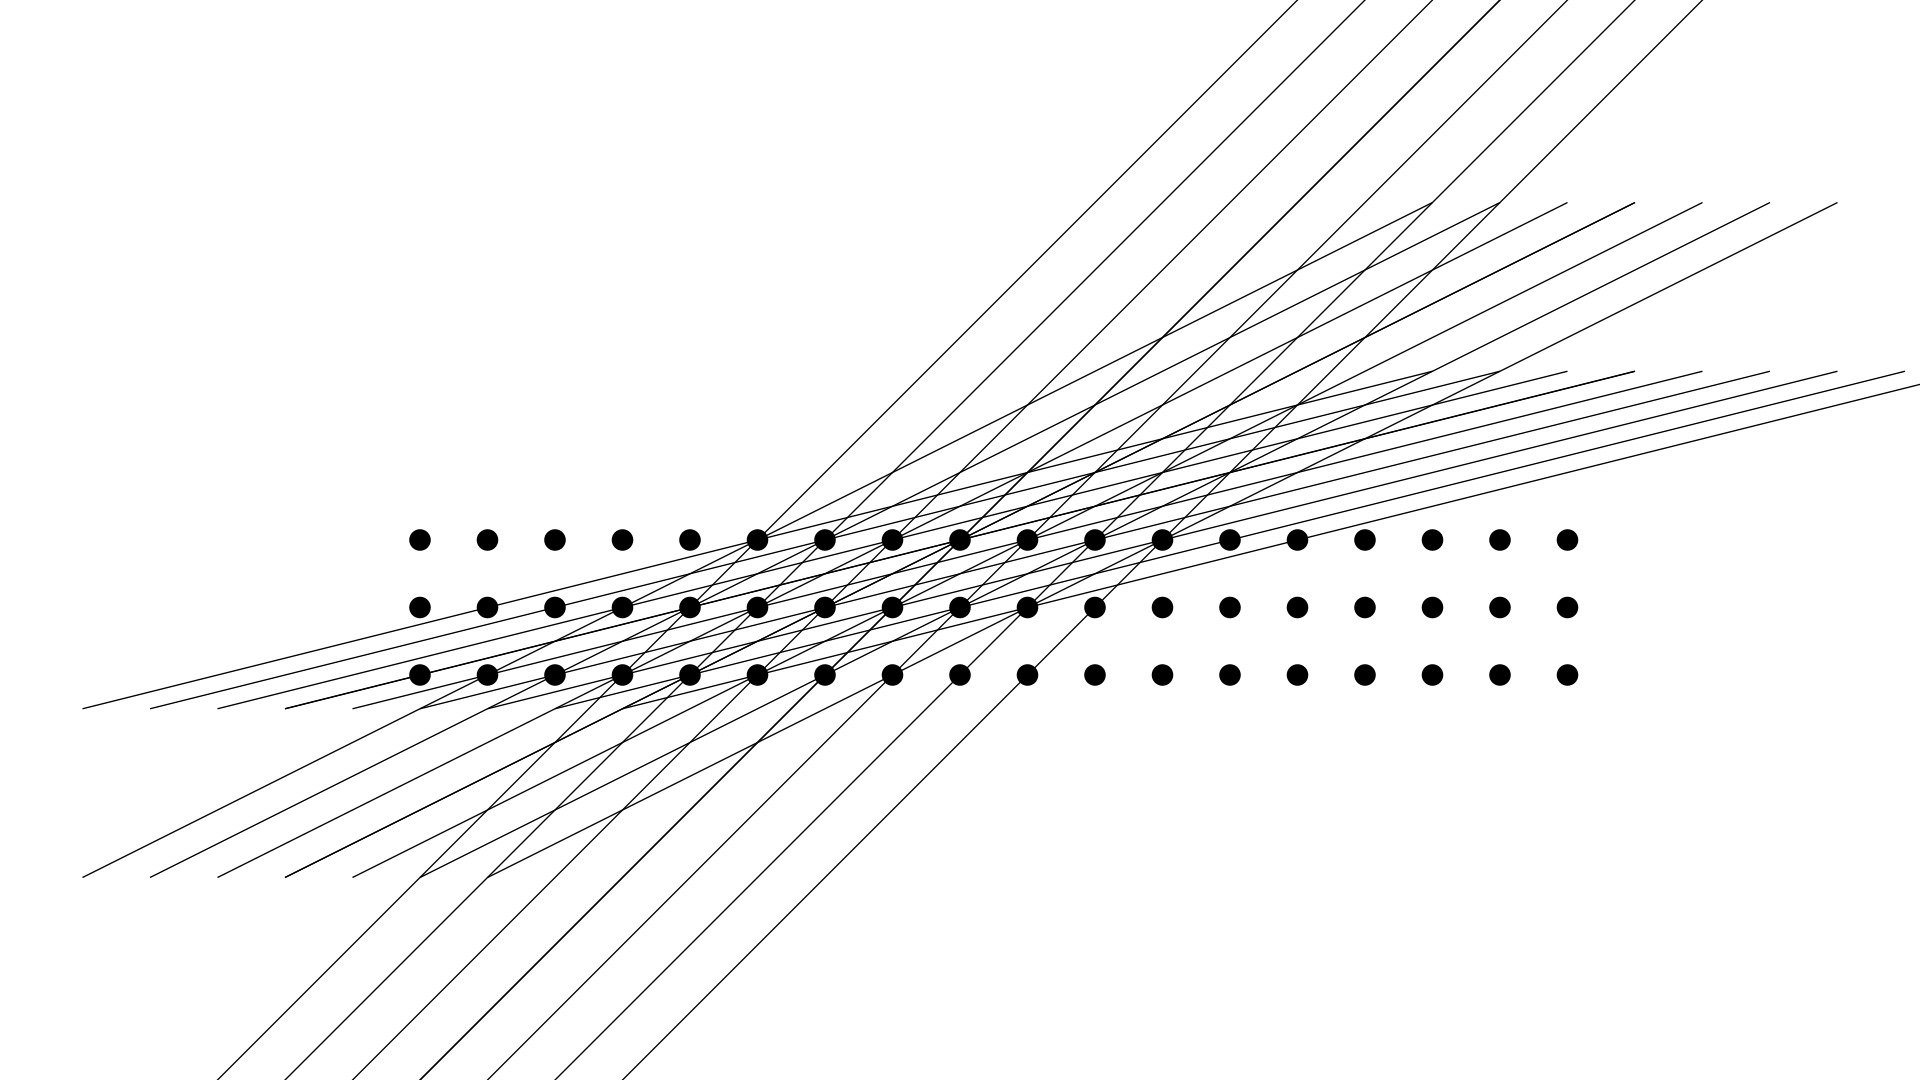
\includegraphics[width=0.8\textwidth]{images/STEX1_ManimCE_v0.15.1.png}
    \caption{Example \ref{ex:ST-1} in the case $N=3$. (with the $x,y$ axis reversed)}
\end{figure}


\begin{example}
    Let $N \gg 1$ be a large even integer and let $1<R \ll N$ be another integer. Consider the collections in $\RR^2$:
    \begin{align*}
        \ES &= \{ (a,b) \in \ZZ^2 \ | \ (a,b) \in [-N/2,N/2] \times [-N/2,N/2] \} \\
        \LL &= \{ \ell \ | \ \ell \text{ contains between R and 2R points of } \ES \} \end{align*}
    We begin by estimating how many lines of $\LL$ pass through a given point of the regular grid $\ES$.
    Let $\ell \in \LL$ and $p \in \ES$. The closest point $p' \in \ES$ such that $p \neq p'$ and $p' \in \ell$ must lie
    in a square centred at $p$ of side length $\sim N/R$. This follows from the fact that there are at least $\sim R$ points of $\ES$ in $\ell$ and hence the
    projections of these points to the axes can be separated by at most $\sim N/R$. Taking each possible combination of these we can conclude that there are $\lesssim N^2 / R^2$ lines in $\LL$ through a
    given point $p$.

    We now claim that there are $\gtrsim N^2 / R^2$ distinct such lines. We need only consider the points in the upper right quadrant of $\ES$ as the problem is symmetrical.
    Further, we restrict ourselves to considering lines with slopes $m$ satisfying $\frac{1}{2} < m < 2$. For such a line to contain $R$  points
    of $\ES$ it is enough that $m= \frac{l}{k} \in \QQ$ with $\gcd(l,k) =1$ and $l,k \in \left[\frac{N}{2R}, \frac{N}{R} \right]$. There are $\gtrsim N^2/R^2$ such pairs ($l,k$), as the proportion of pairs that share a factor of 2 is $\frac{1}{2^2}$ and the proportion of pairs that share a factor 
    of 3 is $\frac{1}{3^2}$, and in general the proportion that shares a factor of $k$ is $\frac{1}{k^2}$. We have that $\sum_{k>1} \frac{1}{k}^2 < \frac{2}{3} < 1$ and hence there are $\gtrsim N^2 /R^2$ distinct
    lines in $\LL$ through each point. Taking account of what we have shown
    \begin{align*}
        |\ES| &\sim N^2, \\ 
        |\LL| &\sim |\ES| \frac{N^2}{R^2} \frac{1}{R} \sim \frac{N^4}{R^3},\\
        |I(\ES, \LL)| &\sim |\ES| \frac{N^2}{R^2} \sim \frac{N^4}{R^2}.\\
    \end{align*}
    we can see that both sides of the \hyperref[thm:S-T]{Szemerédi-Trotter} inequality (Theorem \ref{thm:S-T}) are comparable:
    \[
    |I(\ES, \LL)| \sim \frac{N^4}{R^2} \sim (N^2)^{\frac{2}{3}} \left(\frac{N^4}{R^3}\right)^{\frac{2}{3}} \sim |\ES|^{\frac{2}{3}}|\LL|^{\frac{2}{3}} + |\ES| + |\LL|.
    \]
\end{example}
\todo{add diagram (!)}




\section{Ham Sandwich Theorems \label{sect:ham-sandwich-thms}}
The above examples suggest that the topology of $\RR^2$ plays a key role in this incidence problem. We shall now introduce the method of polynomial partitioning,
which can be seen as the topological analogue to the vanishing lemma (Lemma \ref{lem:kaklem2}) we used in the previous chapters. 

The topological input in the proof will be provided by the following well-known result of Borsuk-Ulam.
Let $\SP^n$ denote the unit $n$-sphere in $\RR^{n+1}$. 
\begin{theorem}[Borsuk-Ulam]
    A map $\phi$ is said to be antipodal if it obeys $\phi (-x) = -\phi(x)$ for all $x$ in its domain. Suppose $\phi: \SP^N \to \RR^N$ is a continuous antipodal mapping. 
    Then the image of $\phi$ contains 0. \label{thm:Borsuk-Ulam}
\end{theorem}
In \hyperref[appendix:Borsuk-Ulam]{the appendix to this manuscript}, we present a beautiful combinatorial proof from Matousek's book \textit{Using the Borsuk-Ulam theorem} (see \cite{matouvsek2003using}).
The proof proceeds by constructively proving the Tucker Lemma, and then using this to imply the Borsuk-Ulam theorem.

Let us now define some useful definitions going forward. 
\begin{definition}[Bisection of a Set]
A function $f :\RR^n \to \RR$ is said to bisect an open set $U$ with volume $\text{Vol}(U) < \infty$ if
\[
    \text{Vol}\{x \in U \ | \ f(x) > 0 \} = \text{Vol}\{x \in U \ | \ f(x) < 0 \} = \frac{1}{2} \text{Vol}(U).
\]
Analogously, a function $f$ is said to bisect a finite set $S$ if both
\[
  |\{x \in S \ | \ f(x) > 0\}| \leq \frac{|S|}{2}   
\]
and 
\[
  |\{x \in S \ | \ f(x) < 0\}| \leq \frac{|S|}{2}.
\]

\end{definition}

We now show that as a consequence of Theorem \ref{thm:Borsuk-Ulam}, it is always possible to find a non-zero continuous function that
bisects every open set in a collection. \todo{check this}
\begin{theorem}[General Ham Sandwich Theorem]
Let V be a finite dimensional vector space of continuous functions $f:\RR^n \to \RR$ such that for any non-zero function $f$,
 $Z(f)$ has zero Lebesgue measure. 
Let $U_1,U_2,\dots,U_N \subset \RR^n$ be finite volume \todo{measure vs vol? I use vol above} open sets with $N< \dim V$. 

Then there exists a non-zero function $f \in V$ that bisects each $U_i$. \label{thm:GenHamSand}
\end{theorem}
\begin{proof}

Define the functions $\{\phi_i\}_{i=1}^N$, $\phi_i: V\backslash \{0\} \to \RR$ by:
\[
\phi_i(f) = \text{Vol}(\{x\in U_i \ | \ f(x) > 0 \}) - \text{Vol}(\{x\in U_i \ |\ f(x) < 0 \}).
\]
Since $Z(f)$ has measure zero, it is easy to see that $\phi_i(f) = 0$ if and only if $f$ bisects $U_i$. 
Notice also that $\phi_i(-f) = -\phi_i(f)$, hence $\phi_i$ is antipodal. 

We now show each $\phi_i$ is continuous.
It is enough to show that if $U$ is a finite volume\todo{is volume fine here?} open set, then the measure of $\{x\in U\ |\ f(x)>0\}$ depends continuously on $f\in V \backslash \{0\}$.

Suppose $f_n \to f$ in $V$ for some $f,f_n \in V \backslash \{0\}$. $f_n$ converges to $f$ in the topology of $V$, 
so it follows it must converge pointwise. Pick any $\varepsilon >0$. 
By Egorov's theorem, we can find a subset $E\subset U$ so that $f_n \to f$ uniformly pointwise on $U \backslash E$ with $m(E)< \varepsilon$.
By hypothesis, $m(Z(f)) =0$ and $m(U) < \infty$. 
Since the Lebesgue measure is continuous we can choose $\delta$ such that $m\left(\{x\in U\ \big |\ |f(x)|<\delta\}\right) < \varepsilon$.

Now we choose $n$ sufficiently large that $|f_n (x) - f(x)| < \delta$ on $U\backslash E$. Then we have by the triangle inequality:
\begin{align*}
    |m&\left(\{x\in U \ |\ f_n(x)>0\}\right) - m\left(\{x\in U\ |\ f(x)>0\}\right)| \\
    &\leq |m\left(\{x\in U\ |\ f_n(x)>0\}\right)| + |m\left(\{x\in U\ |\ f(x)>0\}\right)| \\
    &< 2 \varepsilon. 
\end{align*}\todo{proof is incorrect.}
Since $\varepsilon$ was arbitrary each $\phi_i$ is continuous.

We now combine each $\phi_i$ into the map $\phi : V\backslash \{0\} \to \RR^N$ by $\phi = (\phi_1, \dots, \phi_N)$.
 Since $\dim V > N$, select a subspace $W < V$ such that $\dim W = N+1$. 
Now choose an isomorphism of $W$ with $\RR^{N+1}$, and think of $\SP^N$ as a subset of $W$ \todo{Explain that $\phi$ is actually a function on the unit sphere of V}.
Now the map $\phi: \SP^N \to \RR^N$ is antipodal and continuous. 
By the Borsuk-Ulam theorem, there exists an $f\in \SP^N \subset V\backslash \{0\}$ such that $\phi(f) = 0$.
\end{proof}
We are now going to use the Ham Sandwich Theorem to extend the conclusion to the bijection of finite sets also.
The main idea will be to construct sets of arbitrarily small measure around each of our points in the finite set and apply the previous theorem.\todo{check}
\begin{corollary}[Finite Ham Sandwich Theorem]
    Let $S_1, \dots , S_N$ be finite sets in $\RR^n$ and let $D$ be such that $N < {{D+n}\choose{n}}$. 
    Then there exists a non-zero $P\in \operatorname{Poly}_D (\RR^n)$ that bisects each $S_i$.  \label{thm:FiniteHamSandwich} 
\end{corollary}

\begin{proof}
    Let us equip the space\todo{V or poly Rn?} with the $L^1$ norm.
    For each $\delta>0$, define $U_{i, \delta}$ to be the union of $\delta$-balls centred at the points of $S_i$. 
    By Theorem \ref{thm:GenHamSand}, we can find a non-zero $P_{\delta}$ with degree at most $D$ that bisects each $U_{i, \delta}$. 
    By rescaling we can assume $P_{\delta} \in \SP^M \subset \text{Poly}_D (\RR^n) \backslash \{0\}$.
    Since $\SP^M$ compact, we can find a sequence $\delta_m \to 0$ so that $P_{\delta_{m}}$ converges to $P$ in $\SP^M$.
    Since the coefficients of $P_{\delta_{m}}$ converge t1o those of $P$, $P_{\delta_{m}}$ converges to $P$ uniformly on compact sets.

    We claim $P$ bisects each $S_i$. 
    By contradiction, suppose $P>0$ on more than half the points of $S_i$, say on the points of $S_i^+$. 
    Choosing $\varepsilon$ sufficiently small, we can assume $P>0$ on the $\varepsilon$-ball around each point of $S_i^+$.
    Further, we can choose $\varepsilon$ such that each $\varepsilon$-ball is disjoint. 
    Since $P_{\delta_{m}}$ converges uniformly, we can find $m$ sufficiently large such that $P_{\delta_{m}}>0$ 
    on the $\varepsilon$-ball around each point of $S_i^+$.
    By making $m$ large, we can also arrange that $\delta_m < \varepsilon$.
    Thus $P_{\delta_{m}} > 0$ on more than half the volume of the set $U_{i, \delta_{m}}$, a contradiction. \todo{check}
\end{proof}
We now utilise the above results to prove a powerful cell decomposition technique known as polynomial partitioning.
\begin{theorem}[Polynomial Partitioning]
    If $S$ is a finite subset of $\RR^n$ and $D$ any degree, there exists
    a polynomial $P$ of degree $D$ such that $\RR \backslash Z(P)$ is a disjoint union of \todo{$\sim$ or $\lesssim$}$\sim D^n$ open sets $O_i$ each containing
    $\lesssim_n |S|D^{-n}$ points. \label{thm:PolyPartioning}
 \end{theorem}
 
 \begin{proof}
 The main idea of the proof is the repeated application of the \hyperref[thm:FiniteHamSandwich]{Finite Ham Sandwich Theorem}. We begin by finding a polynomial $P_1$ of degree 1 that bisects $S$. This partitions $\RR \backslash Z(P_1)$
 into two disjoint open sets according to the sign of $P_1$, 
 \begin{align*}
    P_1^+ &= \{ x \in S \ | \ P_1(x) > 0   \} \intertext{and}
    P_1^- &= \{ x \in S \ | \ P_1(x) < 0   \}
 \end{align*}
 each containing at most $|S|/2$ points.
 We then bisect both of these sets using another polynomial $P_2$.
 There are four sign conditions on $P_1$ and $P_2$, these being the four possible intersections of the sets $P_1^{\pm}$ and $P_2^{\pm}$,
 and the subset for each sign condition contains at most $|S|/4$ points of $S$. 
 Continuing this process to define polynomials $P_3, P_4, \dots$, where the polynomial $P_j$ simultaneously bisects $2^{j-1}$ finite sets. 
 By the \hyperref[thm:FiniteHamSandwich]{Finite Ham Sandwich Theorem}, we can find a polynomial of degree $\lesssim 2^{j/n}$ that simultaneously bisects $2^{j-1}$ finite sets.
  
 Repeating this procedure $J$ times, and defining $P = \prod_{i=1}^{J} P_i$, $\RR^n \backslash Z(P)$ is the disjoint union of $2^J$ open sets each containing $ \leq |S|2^{-J}$
 points of $S$. Now we choose $D$ such that $\deg(P) < D$ which is equivalent to $\sum_{j=0}^J c(n) 2^{j/n} \leq D$. But $\sum_{j=0}^J 2^{j/n}$ is a geometric series so we can find $\deg (P) < D$ for $D \leq c(n) 2^{J/n}$. \todo{unsure how to rephrase this}
 The number of points in each $O_i$ is $\leq |S| 2^{-J} \leq c(n) |S| D^{-n}$
 \end{proof}

There is a crucial point to note about polynomial partitioning. 
The above theorem does not guarantee anything about the distribution of points between $Z(P)$ and its complement.
This is made most clear looking at the following two extremes. If all points line in the complement of $Z(P)$ then we have an optimal equidistribution of points,
and can often use trivial bounds in a divide-and-conquer style argument. On the other hand, in the case all points are contained in $Z(P)$ we have
many points in an algebraic surface of controlled degree, so we can try and use tools from algebraic geometry. Generally there will be some points in both $Z(P)$ and its complement
which we need to deal with separately.


\section{Proof of the Szemerédi-Trotter Theorem \label{sect:prf-of-ST}}
We now can prove the \hyperref[thm:S-T]{Szemerédi-Trotter} Theorem using polynomial partitioning.
\begin{proof}[Proof of the Szemerédi-Trotter Theorem]
Let $|\ES| = S$ and $|\LL| = L$. 

Considering the regime where $L > S^2$ and applying the trivial bounds (Lemma \ref{thm:trivial-ST-bounds}) yields
\[
    |I(\ES, \LL)| \leq S^2 + L \sim L \sim (SL)^{2/3} + S + L. 
\] Similarly in the case $L < S^{\frac12}$ we have
\[
    |I(\ES, \LL)| \leq L^2 + S \sim S \sim (SL)^{2/3} + S + L.   
\]
Hence we need only consider the case $S^{\frac{1}{2}} \leq L \leq S^2$.

Let $D$ be a fixed degree to be chosen later. By Theorem \ref{thm:PolyPartioning}, there
exists a polynomial $P$ of degree $D$ such that $\RR^2 \backslash Z(P)$ splits into $\sim D^2$ disjoint open sets each containing $\lesssim SD^{-2}$ points of $\ES$. 
Let $\{O_{i} \ | \ i \in \Pi\}$ denote the family of these components and let $\ES_i = \ES \cap O_i$ and $\LL_i$ denote the lines that intersect the interior of each $O_i$ respectively.
We define the following pairs of complementary sets
\begin{align*}
    \ES_c &=\{x \in \ES \ |\ x \not \in Z(p)\}\\
    \ES_z &=\{x \in \ES \ |\ x \in Z(p)\}\\
    \LL_c &=\{\ell \in \LL \ |\ \ell \not \subset Z(p)\}\\
    \LL_z &=\{\ell \in \LL \ |\ \ell \subset Z(p)\}
\end{align*} 
Note that $\ES = \ES_c \cup \ES_z$, $\LL = \LL_c \cup \LL_z$. We can now write our total line-point incidences as the following sum
$$|I(\ES, \LL)| = |I(\ES_c, \LL)| + |I(\ES_z, \LL_z)| + |I(\ES_z, \LL_c)|.$$
We begin by examining the $I(\ES_c, \LL)$ term
\begin{align*}
|I(\ES_c, \LL)| &= \sum_{i \in \Pi} |I(\ES_i, \LL_i)|.
\intertext{Using our \hyperref[thm:trivial-ST-bounds]{trivial bound} in each cell we attain}
 &\leq \sum_{i \in \Pi} \ES_i^2 + \sum_{i \in \Pi} \LL_i.
\intertext{If a line $\ell$ is not contained entirely in $Z(P)$ then it can intersect $P$ at most $D$ times, 
so each line intersects at most $D+1$ cells. Hence $\sum_{i \in \Pi} L_i \leq (D+1)L$. So we have}
&\lesssim LD + SD^{-2} \sum_{i \in \Pi} S_i\\ &\leq LD + S^2D^{-2}.
\end{align*} 


The number of lines in $\LL_z$ is at most $D$ as $Z(P)$ can contain at most $D$ degree 1 factors.\todo{check} So we have by our \hyperref[thm:trivial-ST-bounds]{trivial bounds} (Lemma \ref{thm:trivial-ST-bounds})
$$|I(\ES_z, \LL_z)| \leq S + D^2.$$
Each line in $\LL_c$ has at most $D$ intersection points with $Z(P)$ so it has at most $D$ incidences with $\ES_z$. Hence:
 $$|I(\ES_z, \LL_c)| \leq LD.$$
Together we have now 
$$|I(\ES, \LL)| \lesssim LD + S^2D^{-2} +S + D^2.$$
We optimise $LD + S^2D^{-2}$ by choosing $D$ such that both terms comparable to each other and hence $D \sim S^{\frac{2}{3}} L^{-\frac{1}{3}}$. 
From our restriction $S^{\frac{1}{2}} \leq L \leq S^2$ we have $S^{\frac{2}{3}} L^{-\frac{1}{3}} \geq 1$
and $D^2 \sim S^{\frac{4}{3}} L^{-\frac{2}{3}} \leq S$, so we achieve
$$|I(\ES, \LL)| \lesssim (SL)^{2/3} + S. $$

Finally combining this with our result for the regime where $L>S^2$ we achieve the full Szemerédi–Trotter inequality 
\[
|I(\ES,\LL)| \lesssim (SL)^{2/3} + S + L.
\]
\end{proof}

There are two key things to note about the above proof. First, the key role that the topology of $\RR^2$ plays. We use topology twice in the above proof. Firstly by using polynomial partitioning, which itself is a consequence of the Borsuk-Ulam theorem from topology. We also appeal to topology in our claim that each line intersects at most $\deg P +1$ components of $\RR^2 \backslash Z(P)$. \todo{check} It is a worthwhile heuristic to develop that polynomial partitioning may be useful for incidence problems
where the best examples in a finite field (which is only equipped with the trivial topology) do not coincide with the best known examples over the reals.
Secondly, the above proof illustrates the surprising power of polynomial partitioning. We were able to use very trivial bounds in each cell to achieve
an asymptotically tight overall bound. 

